\chapter{Sunrise III and TuMag: Design and calibration.}

Observing the Sun with the highest possible quality and resolution is crucial for deepening our understanding of the physical processes governing its behavior. This necessity drives the continuous development of new state-of-the-art observatories and advanced instrumentation. Each new instrument or telescope builds upon the technical achievements of its predecessors, integrating past knowledge while introducing innovations that push the boundaries of solar observation. 

An example of such advancements is the third edition of the Sunrise observatory \citep{SunriseIII}, which marks the culmination of a collaborative effort among several international institutions. Spearheaded by the Max Planck Institute for Solar System Research (MPS) in Göttingen, Germany, the international consortium is also composed by the Spanish Space Solar Physics Consortium (S³PC), the National Astronomical Observatory of Japan (NAOJ), the Leibniz Institute for Solar Physics (KIS) in Freiburg, Germany, and the Johns Hopkins University's Applied Physics Laboratory (APL) in the United States. 

Following an initial unsuccessful flight in 2022, which was aborted six hours after launch, Sunrise III was granted a second opportunity in the summer of 2024. On July 10th, 2024, at 04:22:40 UTC, the observatory was successfully launched by the Columbia Scientific Balloon facility (CSBF-NASA) from Esrange, a scientific facility operated by the Swedish Space Corporation in Kiruna, Sweden. After reaching a stable altitude of about 37.5 km, the commissioning phase began, marking the official start of the observation campaign. Observations commenced shortly thereafter and continued until the campaign concluded on July 16th at 18:20:54 UTC, when the flight was terminated.

Among the payload instruments aboard Sunrise III, TuMag holds particular significance for this thesis. The Tunable Magnetograph (TuMag), is a tunable imaging spectropolarimeter developed by S³PC under the leadership of the Instituto de Astrofísica de Andalucía (IAA-CSIC) in Granada. The S³PC also includes the Instituto Nacional de Técnica Aeroespacial (INTA), the Instituto de Microgravedad Ignacio da Riva (IDR-UPM) from the Universidad Politécnica de Madrid, the Universitat de València (UV), and the Instituto de Astrofísica de Canarias (IAC). TuMag is central to this thesis, as the core of the work focuses on its calibration, operations, and data reduction processes.

In this chapter, we present an overview of the Sunrise III mission, with a particular focus on TuMag. We will first outline the scientific motivations behind its development and the design choices. This will be followed by a detailed discussion of the technical specifications of both the mission and TuMag.

\section{Sunrise III}

Equipped with a telescope with a one-meter aperture, two slit-based spectropolarimeters and an imaging spectropolarimeter, the Sunrise III observatory is the most complex solar telescope to ever leave the ground. The coordination of three different scientific instruments allows Sunrise to simultaneously perform narrow-band polarimetric imaging in the visible while carrying out spectropolarimetry in the near-UV and near-IR, from the advantageous point of observation at $\sim$36 km of altitude leaving behind the Earth atmosphere's turbulence. 

The three instruments aboard Sunrise III have been carefully designed to complement each other and address the scientific purposes of the mission. TuMag carries out high-spatial-resolution imaging spectropolarimetry in the visible range of light. Able to tune to three different spectral lines, namely the highly Zeeman-sensitive Fe I lines at 525.02 and 525.06 nm, and the Mg I b$_2$ line, TuMag can probe the photosphere and low chromosphere quasi-simultaneously. The absence of atmosphere allows the Sunrise Spectropolarimeter and Imager (SUSI, \citealt{susi}), developed by MPS and NAOJ, to observe in the near-UV, performing imaging and spectropolarimetry in the range of 309-417 nm. The high polarimetric sensitivity and large number of spectral lines present in this range, many of which are sensible to the Hanle effect, allows SUSI to sample many heights in the solar atmosphere at the same time while measuring the weak magnetic fields. The Sunrise Chromospheric Infrared spectro-Polarimeter (SCIP, \citealt{SCIP}), co-developed by NAOJ and S³PC, also takes advantage of the absence of atmosphere and observes two of the Ca II triplets lines, and the upper photospheric K$_{1}$ lines close to 770nm, which are poorly accesible from ground. Spectropolarimetry measurements of these lines provides information of the 3-D structure of the chromosphere and its magnetic fields, derived thanks to the high Zeeman sensitivity of the selected lines. Furthermore, the large number of available photons at these wavelengths ensures a high S/N and polarimetric sensitivities. 

The ability to probe simultanously the near-IR, the visible and the near-UV, performing high-resolution polarimetric imaging and spectroscopy makes Sunrise III a unique observatory, capable of studying the connection  and interaction of the small-scale phenomena ocurring at different layers of the solar atmosphere with unprecedented detail and completeness. 

\begin{figure}[t]
    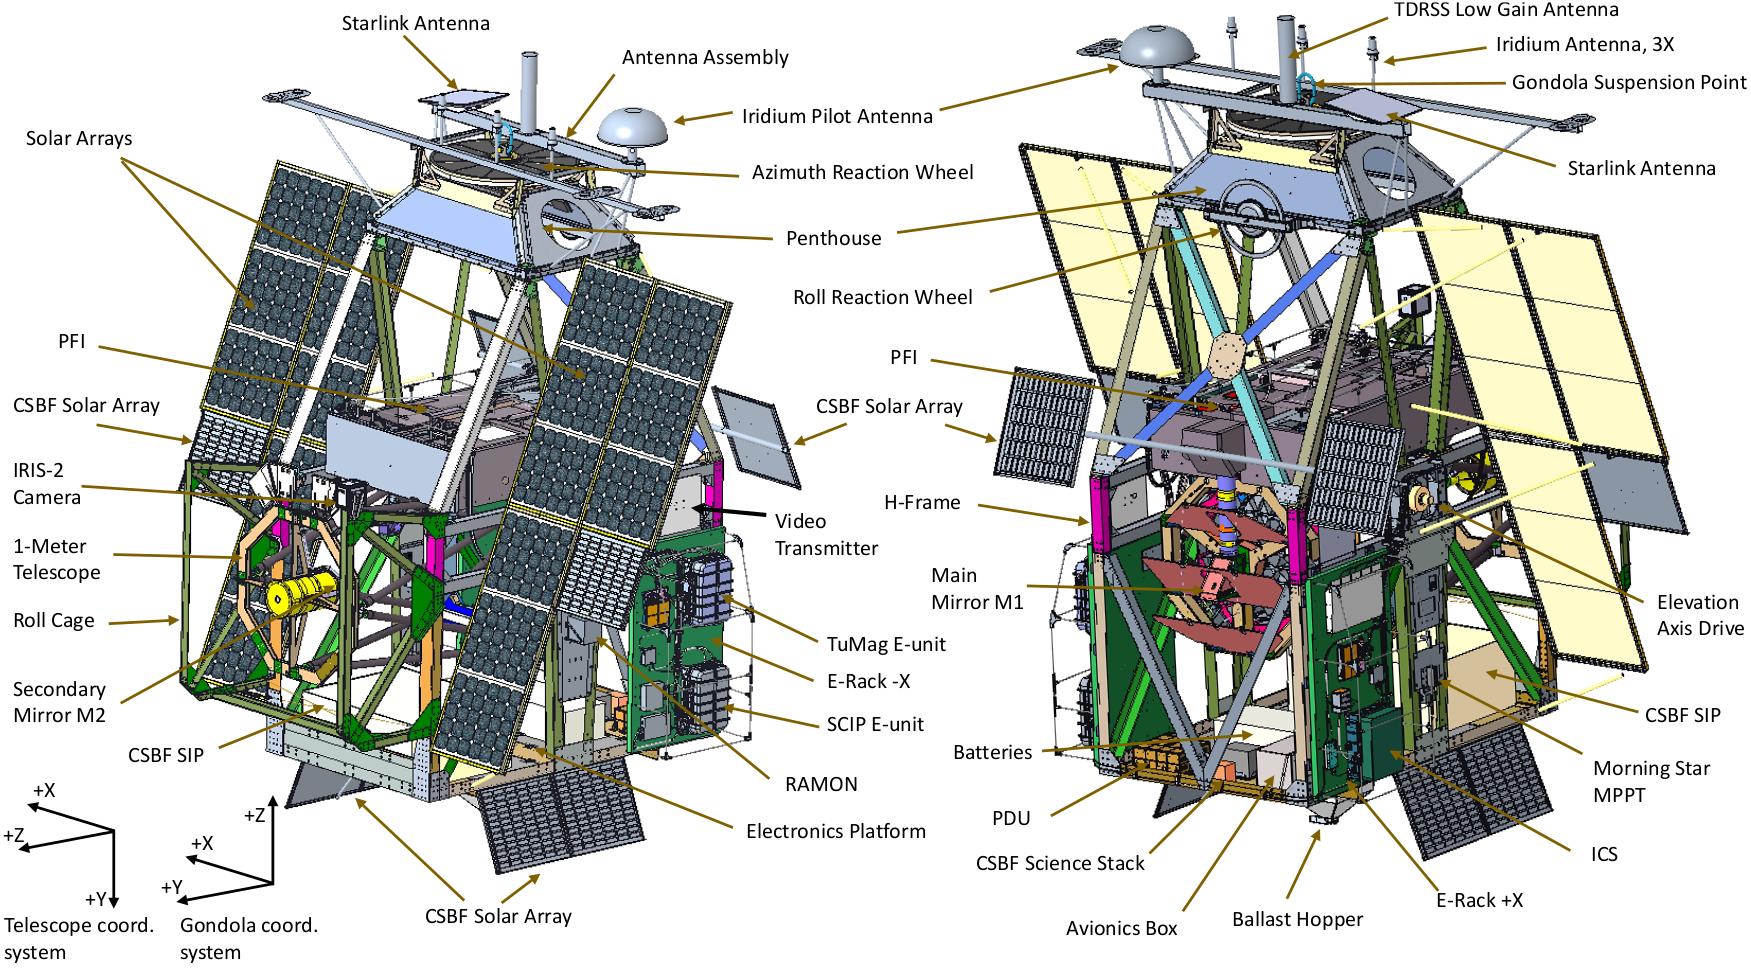
\includegraphics[width=\textwidth]{figures/TuMag/Sunrise_schematic.png}
    \caption[Sunrise III observatory design.]{
      Drawing design of the Sunrise III observatory. Image reproduced from \citep{SunriseIII} with permission, courtesy: APL, P.Bernasconi.}
      \label{fig: SunriseIII}
\end{figure}

\subsection{Observatory's design}

While the scientific instruments are central to the research performed by Sunrise, several additional subsystems play a crucial role, each contributing to the overall success of the mission.

The structural framework housing all components of the observatory, as well as the interface connecting the observatory to the flight apparatus, is provided by the gondola. This gondola, engineered by APL, is not only tasked with safeguarding the instruments and telescope during ascent and landing, but also with ensuring the stability of the pointing system. Given that the observatory is suspended from a balloon, it is subject to wind-induced motion and pendulum-like oscillations, which threaten the stability required for prolonged observations. The gondola pointing control system (PCS) must actively counteract these disturbances in real time by making precise adjustments to the telescope elevation and azimuth. In conjunction with the Correlating Wavefront Sensor (CWS), developed by KIS, which is responsible for image stabilization and autofocus, the full pointing system was required to achieve a pointing accuracy better than 0.005" root mean square (rms) over extended periods to facilitate long-duration observations.

The Sunrise III telescope is a Gregory-type reflector with a 1-meter aperture, featuring a 234 mm central obscuration and an effective focal length of 24.2 meters. This configuration provides a field of view (FoV) of 3.4', corresponding to approximately 150 Mm on the solar surface. The telescope directs light to the post-focus instrumentation platform (PFI), located above the telescope. The PFI houses the three scientific instruments and the CWS, and is responsible for distributing light among these four instruments. This distribution, performed by the Image Stabilization and Light Distribution Unit (ISLiD), must efficiently separate the different wavelengths in a photon-efficient manner to provide the highest number of available photons to each instrument. 

While all the subsystems discussed thus far directly influence the optical performance, it is equally important to recognize the crucial role played by other subsystems, such as the electronics and software control. In particular, the Instrument Control System (ICS) is responsible for the management of the observatory, gathering housekeeping and issuing commands to the electronic units of each instrument. As will be elaborated in the following chapter, Sunrise III observations were designed to operate in a semi-autonomous manner through the use of pre-programmed timelines. This approach requires that all electronic systems function in synchrony, with minimal human intervention. 

\subsection{Science with Sunrise}

The absence of Earth's atmosphere opens the window for simultanous observations in the near-UV, the visible, and the near infrared, and offers a level of image stability that cannot be achieved in ground-based observatories due to atmospheric seeing. However, these advantages are also present in spaceborne missions, such as the Hinode mission \citep{Hinode} and its Solar Optical Telescope \citep{sot}, or the the Solar Orbiter mission (SO; \citealt{SO}) and the Polarimetric and Helioseismic Imager (SO/PHI; \citealt{PHI}), among many others. Nonetheless, spaceborne missions have strong restrictions regarding payload, mass and data rate. 

The absence of these restrictions in balloon-borne observatories often allows for more complex and versatile instrumentation compared to space missions and at a significantly lower budget. The combination of these two factors, namely the absence of atmosphere and the complex and advanced instrumentation they can carry, places observatories such as Sunrise in a unique position, and provides them with splendid perspectives on solar phenomena.

Many aspects of the physical processes driving our Sun remain unsolved. The mechanisms underlying various solar phenomena are still the subject of debate, ranging from the origin and removal of magnetic flux in the solar photosphere to the processes responsible for heating the chromosphere and corona, as well as the small-scale dynamics of solar plasma. The three instruments aboard Sunrise work in consonance to provide novel insights into these phenomena, and aim at helping the community solve some of the open questions in solar physics. In particular, the spectropolarimetry carried out in different spectral ranges allows for the deduction of the structure of the vector magnetic field at different heights. 

The magnetic field, present across multiple scales and heights, is the principal driver of solar activity. Understanding the magnetic field is essential for comprehending the processes that govern solar phenomena, energy distribution, and plasma dynamics. Numerous studies have focused on the investigation of magnetic field structures and their evolution. For example, extensive research has been dedicated to examining the processes responsible for the emergence and cancellation of magnetic flux in the quiet Sun photosphere. These studies propose various models to explain these processes; however, current observations do not definitively favor any particular model.

A thorough 3-dimensional analysis of the magnetic fields throughout the solar surface, from the quietest areas to active regions, is essential to determine how the magnetic field is structured across the solar atmosphere. The combination of spectropolarimeters and vector magnetographs aboard Sunrise, which are capable of measuring magnetic fields through the Zeeman effect, and of detecting the weakest and more turbulent \citep{quiet_sun_living_review} magnetic fields present in the solar surface using the Hanle effect - particularly in the UV - can provide a completely new perspective about how the magnetic field is structured 

In addition to the study of magnetic field structures, Sunrise III aims to study the upper atmosphere, whose dynamics and heating mechanisms are not yet completely understood. In fact, the transfer of energy from the lower layers to the chromosphere and corona is one of the open problems in stellar astrophysics. Several studies propose mechanisms in which the magnetic field plays a central role in this energy transfer. Some works suggest upward currents generated by the slow motion of plasma in the photosphere as a driving mechanism (\citealt{upwards1}, \citealt{upwards2}), while others highlight heating processes induced by jets \citep{jetscorona} or magnetic vortex phenomena, such as twisted magnetic fields known as solar tornadoes \citep{solar_tornadoes}.

Although some observational signatures of these processes have been detected, the detailed characterization of these events requires higher spatial and temporal resolutions than those currently available. The high-cadence UV observations, where several spectral lines sensitive to the weaker magnetic fields of the chromosphere are present, combined with magnetic field maps of the photosphere and lower chromosphere provided by TuMag, and complementary observations of the Ca II infrared lines, provide Sunrise with the necessary tools to investigate these phenomena with unprecedented detail.

Sunrise will also provide novel insights into small-scale plasma dynamics. The Sun is highly dynamic, with structures evolving on timescales of minutes. Several studies propose that the magnetism in the quiet Sun is driven by the turbulent small-scale dynamics of the plasma (\cite{small_scale_dynamo}, \cite{small_scale_dynamo_2}, \cite{small_scale_dynamo_3}, among others). However, investigating these processes requires high spatial and temporal resolutions, which are often unattainable in ground-based observations. Similarly, other approaches to plasma dynamics, such as helioseismology \citep{helioseismology}, also demand such high-resolution data. To address these challenges, Sunrise III conducted extended, highly stable due to the absence of atmospheric seeing, and uninterrupted observations lasting up to six hours, with the highest temporal resolution permitted by the S/N requirements.

In addition to these objectives, Sunrise will explore new and exciting areas, including the measurement of the polarized solar spectrum in the UV. This spectral region remains largely unexplored due to the technical challenges associated with its observation. Atmospheric absorption makes it impossible to observe this band from ground-based observatories, and it has yet to be measured by any space mission at the resolutions provided by a one meter telescope and with a high sensitive spectropolarimeter. SUSI is the first UV spectropolarimeter to acquire such high-resolution data in this wavelength range.

\section{The Tunable Magnetograph: TuMag}

\begin{table}
    \centering
   \begin{tabular}{cc}
    \hline
    \hline
    Requirements & Value \\
    \hline
    Field of view & $63''$ x $63''$ \\
    RMS wavefront error & $W \sim \lambda / 14$\\
    Spatial sampling & $3 \times 3 $ pixels \\
    Plate scale & $0.0378''$ / pixel \\
    Polarimetric efficiencies & $\epsilon _ {1, 2, 3} \lessapprox \frac{1}{\sqrt{3}}$\\
    S/N ratio & $\left(\frac{S}{N}\right) _ 0 \gtrapprox 1700$ \\
    Spectral resolution & $< 9$ pm\\  
    Spectral lines & Fe I 5250.2 \r{A}, Fe I 5250.6 \r{A}, and Mg I $b_2$ 5172.7 \r{A}. \\
    Time for a two-line observation & $< 90$ s\\
    \hline
    \hline
    \end{tabular}
    \caption{Tumag scientific requirements.}
    \label{table: Tumags requirements}
\end{table}

TuMag is an FPI-based tunable imaging spectropolarimeter, capable of measuring the full Stokes vector across various spectral lines over a bidimensional zone of the Sun. This tunability allows TuMag to probe the magnetic field in both the photosphere and lower chromosphere, with high resolving power, thanks to its near-diffraction-limited imaging capabilities. Key technologies of TuMag are inherited from IMaX \citep{IMaX}, the imaging spectropolarimeter that flew aboard previous Sunrise missions. However, TuMag incorporates several advancements over its predecessor, including the addition of filter wheels for tunability between three different spectral lines and the ability to introduce several calibration targets to the observations, along with newly designed cameras and modulation packages. Additionally, all software and firmmware has been completely redone for TuMag, including the ground segment software, GUIMAG.

In this section, we present an overview of the design of TuMag  and its performance. It is important to note that this discussion will primarily focus on the instrument optical performance—specifically its polarimetric, spectral, and imaging properties. Other aspects, such as the thermal behaviour, the electronics or the control software, among others, while crucial to the instrument's functionality, will not be covered here to avoid excessive length. Many of these aspects can be found in the TuMag paper \citep{tumag}.

\subsection{TuMag's design and light path.}

As a polarimeter, TuMag must be able to measure the full Stokes vector of the incoming light. To achieve this, it must generate four distinct modulation states and measure them in an almost simultaneously manner. As a spectrometer, TuMag must possess the capabilityfor selecting specific wavelengths along multiple spectral lines. This process involves, first filtering the light with a pre-filter, which selects a "broad" spectral range, followed by an etalon that further narrows the bandpass within the selected range. Throughout this procedure, stringent requirements regarding polarimetric sensitivity (efficiency), spectral resolution, and imaging quality must be maintained. A summary of these requirements is presented in Table \ref{table: Tumags requirements}.

\begin{figure}[t]
    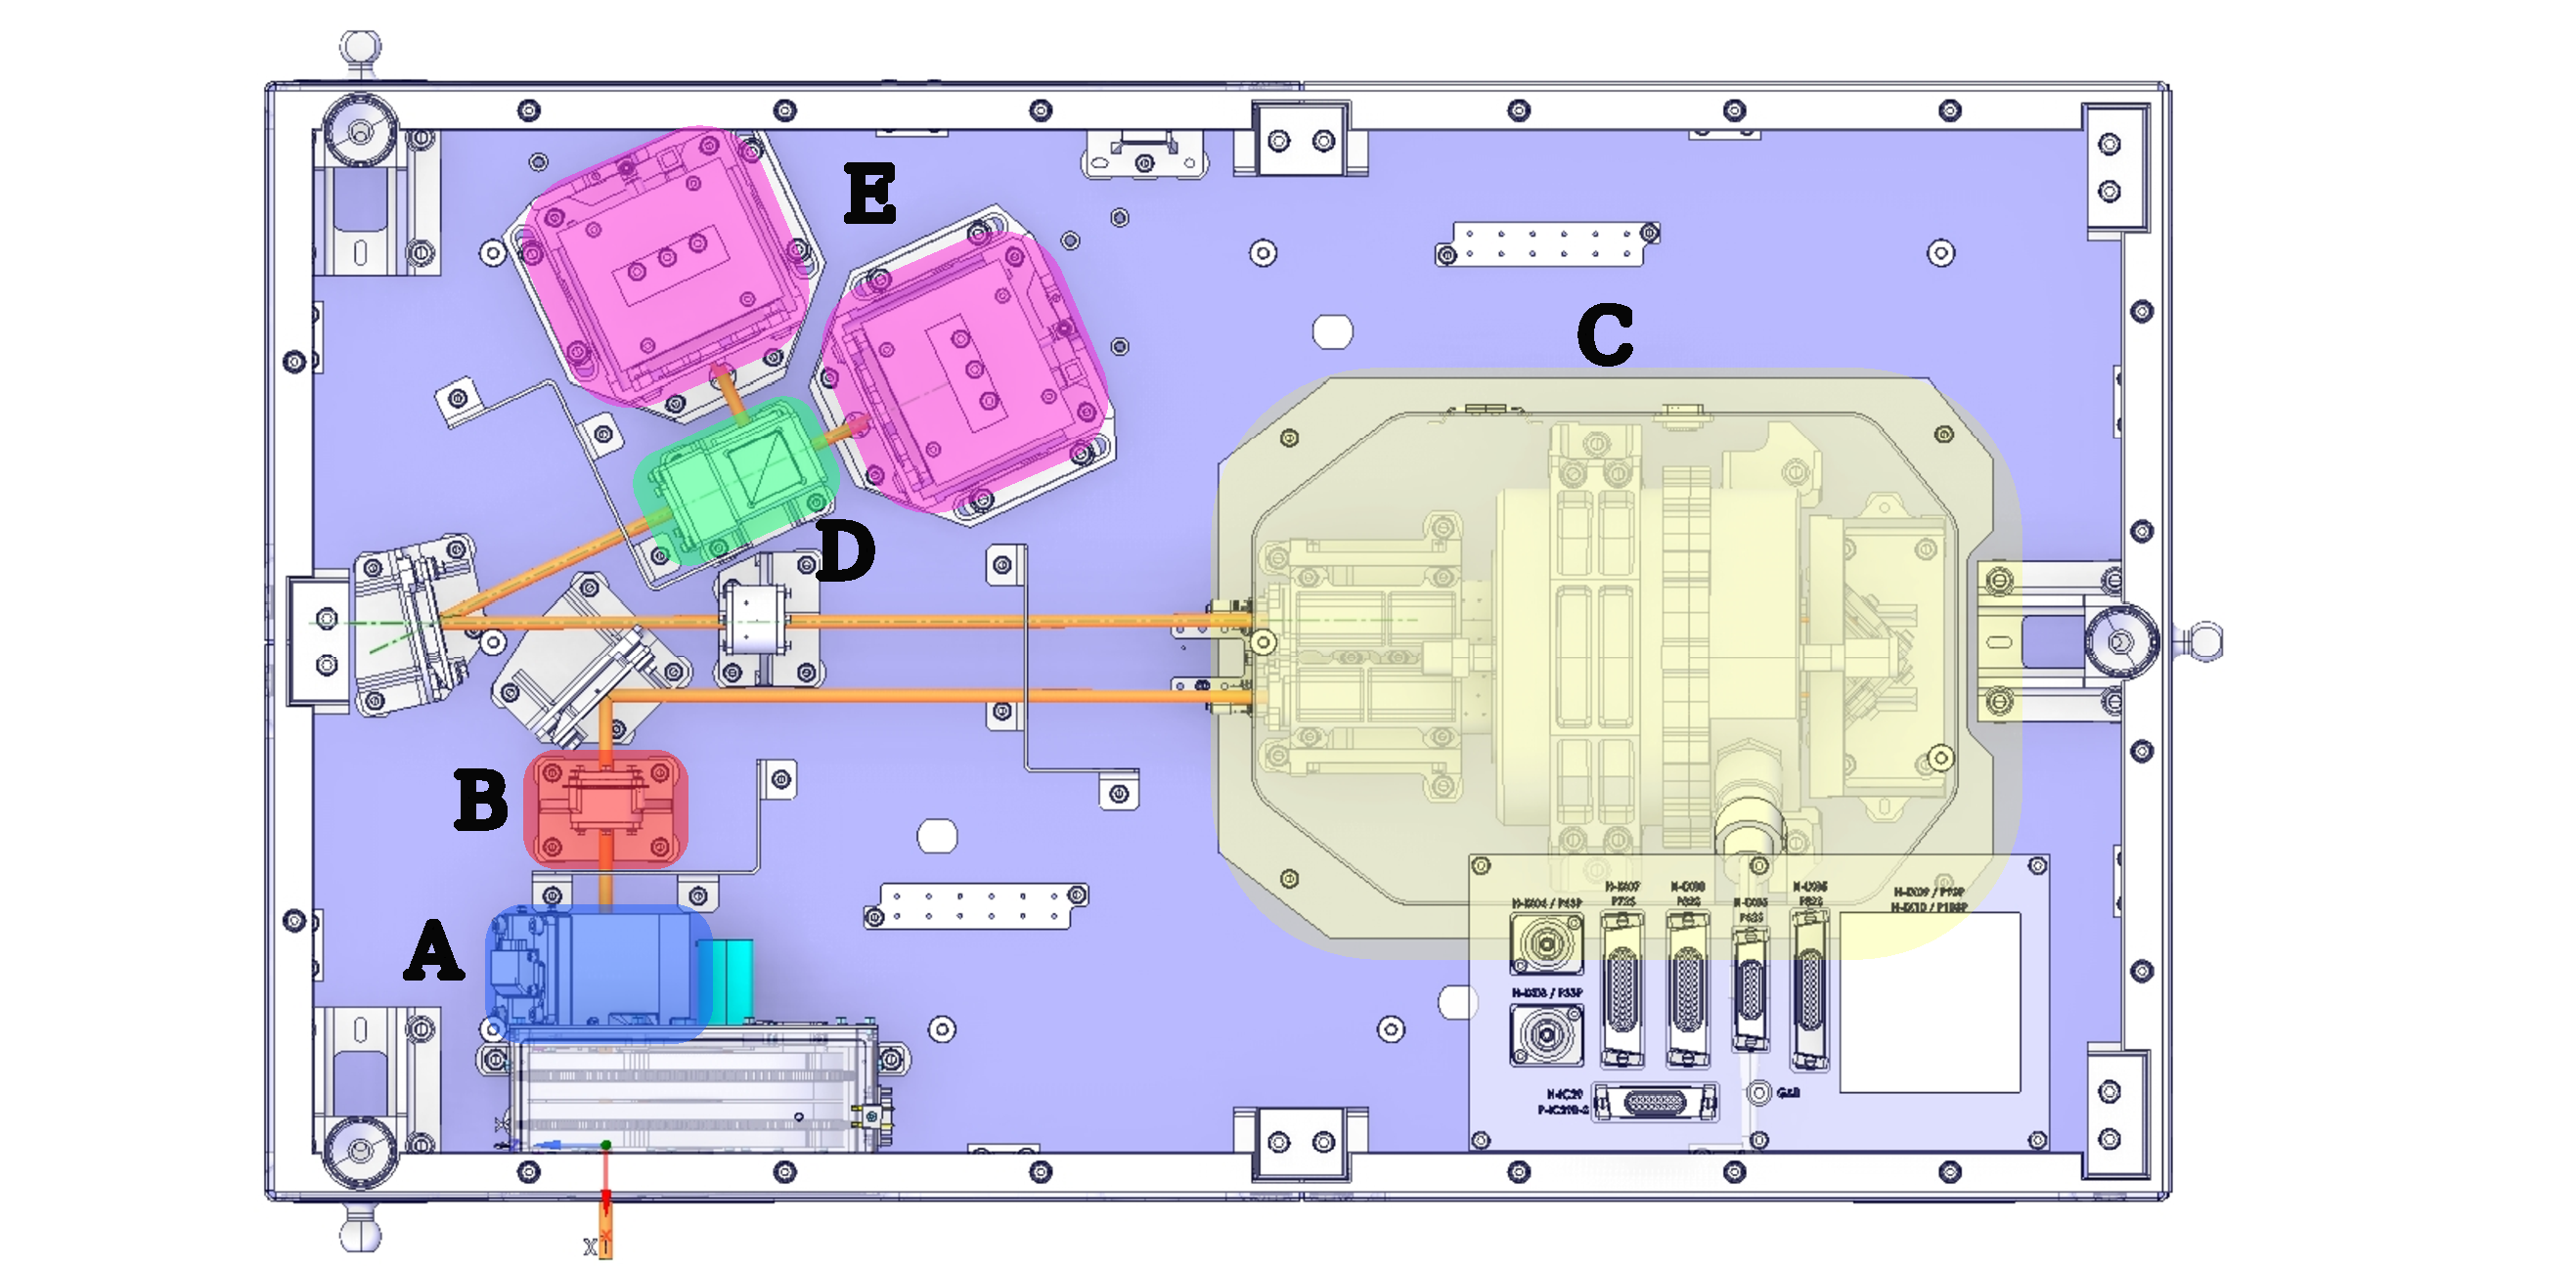
\includegraphics[width=\textwidth]{figures/TuMag/Scheme.pdf}
    \caption[Tumag schematic.]{Schematic representation of the Tumag instrument. Some relevant optical devices in the light path (yellow line) are highlighted with a colored box and labeled with letters from A to E: A) Filter wheel, B) PMP, C) Etalon oven, D) beam-splitter and E) cameras. Image taken from \cite{tumag}, reproduced with permission.      
    \label{fig_tumag:scheme}}
\end{figure}

Light is delivered to TuMag by the ISLiD system and subsequently re-imaged onto two cameras where the images are recorded. Before reaching the cameras, the light passes through all the different subsystems of the optical unit. The first components encountered by the light are a blocking prefilter and the filter wheel (box A in Fig.~\ref{fig_tumag:scheme}). The blocking prefilter, with a wide bandpass centered at 520 nm, is employed to eliminate unwanted spectral ranges. The filter wheel is comprised by a double-disk system \citep{filter-wheels} that houses the prefilters for selecting specific spectral lines and a series of calibration targets. Specifically, the first disk carries a linear polarizer, a plate of micropolarizers, a pinhole set and a phase diversity (PD) plate. The latter consists on a plane-parallel plate of $1.45 \lambda$ of width \citep{fran-pd} that introduces a known defocus into the image, allowing for phase diversity computations. The second disk hosts the three pre-filters, corresponding to the spectral lines Fe I 5250.2 \r{A}, Fe I 5250.6 \r{A}, and Mg I $b_2$ 5172.7 \r{A}, in addition to a dummy target that can be employed to allow all spectral ranges to enter the instrument.

After passing through the filter wheels, the light is directed into the Polarization Modulation Package (PMP) \citep{pmp1}, highlighted with the red box in Fig.\ref{fig_tumag:scheme}. The PMP primary function is to modulate the light in order to produce the different polarization states required to deduce the Stokes components. This is achieved using two liquid crystal variable retarders (LCVRs), which are oriented with their fast axes at 45$^\circ$ relative to each other. These LCVRs induce a retardance on the transmitted light that varies with the voltage applied across the crystals. The system can operate in two distinct modulation schemes: a vector modulation scheme, which generates four independent linear combinations of, ideally, equally-weighted Stokes components across consecutive observations, allowing for the retrieval of the full Stokes vector after demodulation; and a longitudinal modulation scheme, which generates only two modulations, providing information solely on the intensity and circular polarization.

Following modulation, the light is directed into a LiNbO$_3$ Fabry-Pérot etalon, highlighted in yellow in Fig.\ref{fig_tumag:scheme} (box C). Likewise IMaX, the etalon operates in a collimated setup and with a double pass configuration \citep{etalon-doublepass}. In this configuration, after the light passes through the etalon once, it is redirected by a pair of mirrors to pass through the etalon a second time. This double-pass configuration significantly enhances spectral resolution by narrowing the transmission profile. The LiNbO$_3$ etalon tunes the resonance wavelength by varying the refractive index of the cavity through the application of high voltages (ranging from $-4000$ V to $4000$ V). Compared to air-gapped etalons, these kind of etalons offer the advantage of having no moving parts, which is particEEEularly beneficial for spaceborne or balloon-borne instruments. However, this advantage comes with the need for precautions to prevent discharges caused by air ionization.

The final optical element the light encounters before reaching the cameras is a polarizing beam splitter (green box in Fig.\ref{fig_tumag:scheme}). At this stage, the light beam is divided into two orthogonal, linearly polarized components, each directed towards a different camera. This dual-beam configuration \citep{lites-doublebeam} is designed to minimize spurious signals induced by jitter of the gondola (see \citealt{libro_JoseCarlos} for an extended discussion), as it effectively cancels fluctuations from Stokes I to the other Stokes parameters that may arise due to image motion or solar evolution (\textit{i.e.}, cross-talk).

Light then reaches the two custom-made cameras (boxes E; \citealt{tumag-cams} equipped with GPIXEL back-illuminated GSENSE400BSI detectors, each featuring a $2k \times 2k$ pixel array, and specifically designed to meet TuMag's scientific requirements. These cameras accomodate a FoV of $63'' \times 63''$, sufficient to encompass an entire medium-sized active region, with a plate scale of $0.0378''$/pixel.

After mission recovery, the data are processed on-ground to combine images from the different cameras, modulation states, and spectral lines, ultimately deriving the scientific products. This processing and reduction of the data is accomplished using software specifically developed for TuMag, which will be extensively discussed in Chapter \ref{CH:Pipeline}. 

\subsection{Instrument performance and verification.}

To ensure data quality, TuMag underwent multiple verification and calibration processes, during which its spectral, polarimetric, and imaging properties were meticulously tested. These tests, commonly referred to as end-to-end (E2E) calibration tests (see \cite{e2e-tests-inta} for a detailed description of the tests), were conducted at various stages during the development of TuMag. Specifically, they were performed during the assembly, integration, and verification (AIV) activities with the stand-alone instrument at INTA facilities in Madrid, Spain; during the AIV phase of the PFI platform at MPS facilities in Göttingen, Germany; and during the TuMag AIV phase in the Sunrise III mission at ESRANGE facilities in Kiruna, Sweden. These tests were designed not only to validate the instrument capabilities but also to measure critical parameters such as the tuning constant of the etalon, modulation matrices, and best-focus position—each of which is vital for the optimal operation of TuMag and the subsequent data processing. We will now delve into the details of the imaging, spectral and polarimetric properties of the instrument as well as the verification processes and results.

\subsubsection{Imaging performance.}

The imaging E2E tests involved projecting several targets at the F4 focus, including an USAF test target, star targets, and a grid, observed both with and without the PD plate. These targets were utilized to evaluate the MTF and to assess the resolving power of TuMag. The PD measurements enabled verification of the wavefront error (WFE) derived from the MTF and an evaluation of the image quality following image restoration. 

The USAF target \footnote{The 1951 USAF target from Thorlabs Inc, model: R1DS1N.} consists on a series of horizontal and vertical line pairs (lp) arranged in sets of three with varying resolutions. Identifying the highest resolution group observable with TuMag allows for a fast diagnostic of the instrument resolution and performance. In Fig.~\ref{tumag : USAF}, measurements of group 4 and 5 (and higher) of the USAF target are shown for both cameras and the three pre-filters. The second set of group 5 (highlighted in a white box), which corresponds to 35.9 lp/mm in the target and 24.3 lp/mm in the image, is of special interest since its close to the Airy disk radius (26.4 lp/mm) and therefore close to TuMag's resolution limit. 

\begin{figure}[t]
    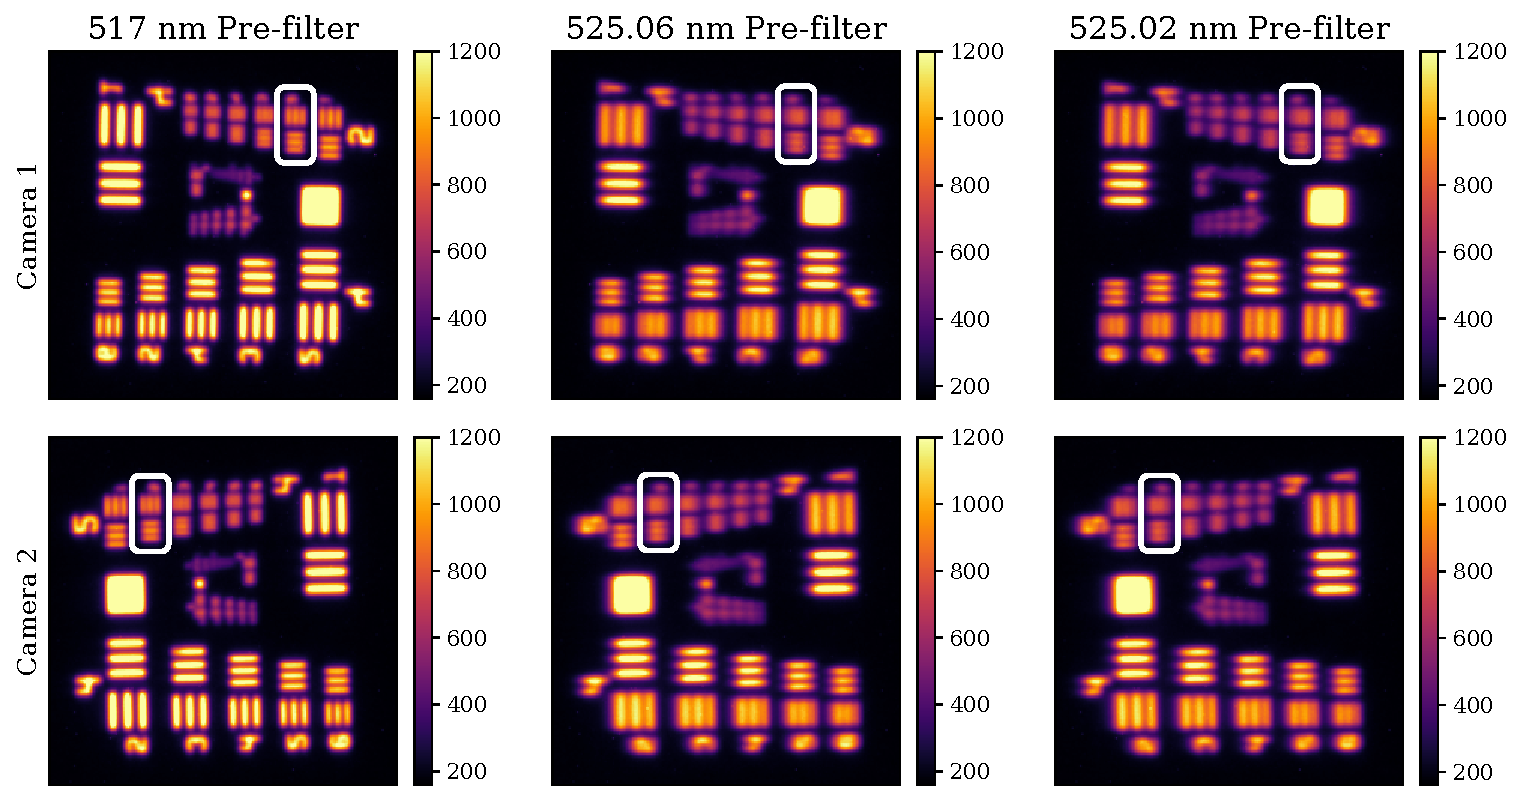
\includegraphics[width=\textwidth]{figures/TuMag/USAF_E2E.pdf}
    \caption[Optical E2E USAF measurements.]{
      USAF target measurements for both cameras and the three pre-filters performed during E2E tests at INTA facilities on December 2021. The white boxes highlight the second element of the test group 5 (35.9 lp/mm). The scale of the images is set in digital counts.}
      \label{tumag : USAF}
\end{figure}

The results show a better optical performance for the 517 nm pre-filter than the other two pre-filters. The USAF 5.2 set is clearly resolved for this pre-filter in both cameras showing almost no difference between vertical and horizontal resolutions. However, results for the 525 nm prefilters exhibit a worsening of the resolution, with the same set being hardly resolved in the horizontal direction in both prefilters. 

\begin{figure}[t]
    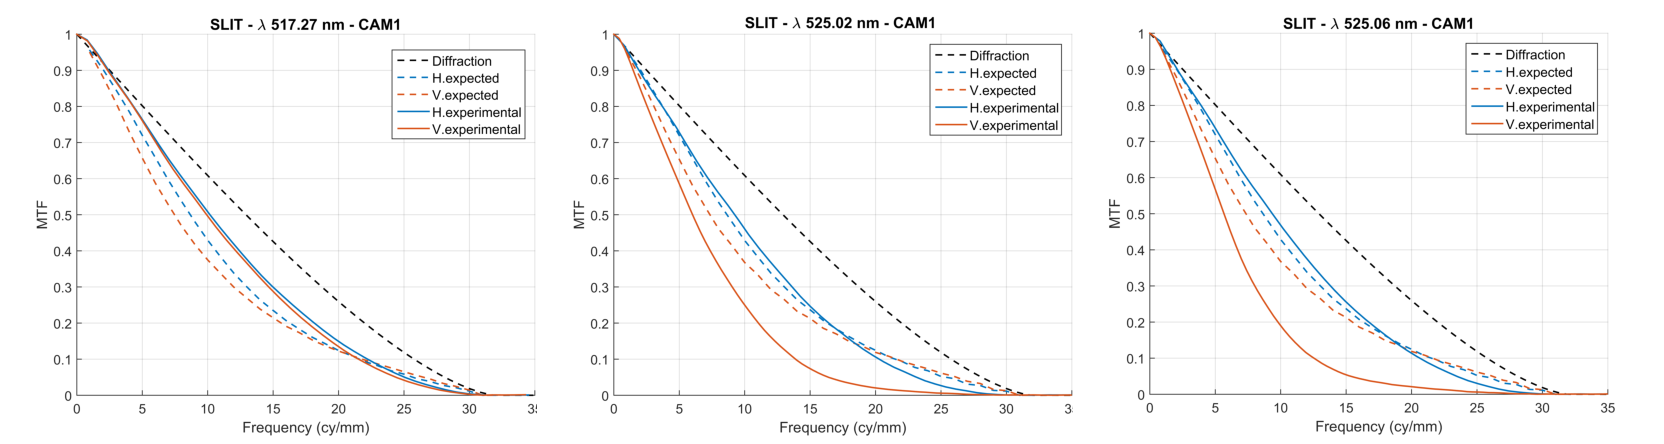
\includegraphics[width=\textwidth]{figures/TuMag/mtfs.pdf}
    \caption[TuMag's MTFs.]{MTFs derived for camera 1 (very similar results for camera 2) for the three pre-filters from measurements of the stand-alone AIV phase performed at INTA in December 2021. Image taken from \citep{tumag}, reproduced with permission. Analysis performed by INTA. 
      \label{fig_tumag:mtfs}}
\end{figure}


However, a more precise evaluation of the optical performance can be achieved from the MTFs. Figure \ref{fig_tumag:mtfs} shows the MTFs computed with a slit target (see \citealt{slanted-method} for a description of the MTF computation method) during the E2E tests performed in December 2021 at INTA facilities. These results agree with the diagnostic carried with the USAF tests: the 517 nm pre-filter shows a good performance in both directions, with values above the expected behaviour. Meanwhile, 525 nm pre-filters exhibit a large difference between different directions with an important drop in vertical resolution in both cases. This observed astigmatism is attributed to the etalon and physical deformations of the pre-filters caused by the mechanical method used to secure and tilt them. This effect is particularly noticeable in the iron pre-filters due to the higher angles of incidence required for their tuning.

\begin{table}[t]
    \centering
   \begin{tabular}{ccccc}
    \hline
    \hline
    Pre-filter and & Strehl ratio & Strehl ratio & $W_{\text{rms}}$& $W_{\text{rms}}$\\
    camera & Vertical & Horizontal & Vertical & Horizontal\\
    \hline
    517 nm - Cam 1 & 0.782 & 0.826 & $\lambda/12.7$ & $\lambda/14.5$ \\
    517 nm - Cam 2 & 0.761 & 0.806 & $\lambda/12.1$ & $\lambda/13.5$ \\
    525.02 nm - Cam 1 & 0.436 & 0.725 & $\lambda/6.9$ & $\lambda/11.1$ \\
    525.02 nm - Cam 2 & 0.405 & 0.726 & $\lambda/6.6$ & $\lambda/11.1$ \\
    525.06 nm - Cam 1 & 0.451 & 0.764 & $\lambda/7$ & $\lambda/12.1$ \\
    525.06 nm - Cam 2 & 0.444 & 0.736 & $\lambda/7$ & $\lambda/11.3$ \\
    \hline
    \hline
    \end{tabular}
    \caption{Optical performance evaluated from the MTFs obtained with the slit target at December 2021 E2E tests. Results taken from \citep{e2e-tests-inta}.}
    \label{table: Optical-performance}
\end{table}


The comparison of the obtained MTF and the diffraction-limited one allows for an estimation of the Strehl ratio, and consequently the wavefront error (see section \ref{sec: intro-imaging}).

Table \ref{table: Optical-performance} shows the results for the Strehl ratios and $W_{\text{rms}}$ derived from this computation. All values, except for the horizontal resolution in camera 1 of the 517 nm pre-fiter are lower than the $\lambda/14$ set as a requirement. However, in order to enhance the optical performance of the instrument, TuMag is equipped with a PD plate in the filter wheel that allows for the assessment of the PSF during the observations to apply image restoration techniques during the data processing. Through this reconstruction, the images can remove the additional aberrations introduced by the telescope, the image stabilization and light distribution (ISLiD) system and uncorrected jittering. Images can always be restored if $W_{\text{rms}} \gtrapprox \lambda / 5$ \citep{vargas_tesis} if the PSF is known. Furthermore, PD techniques not only allow us to enhance the optical performance of the instrument but also evaluate the optical performance during the calibrations in order to verify the results obtained through the computation of the MTF. 

\begin{figure}[t]
    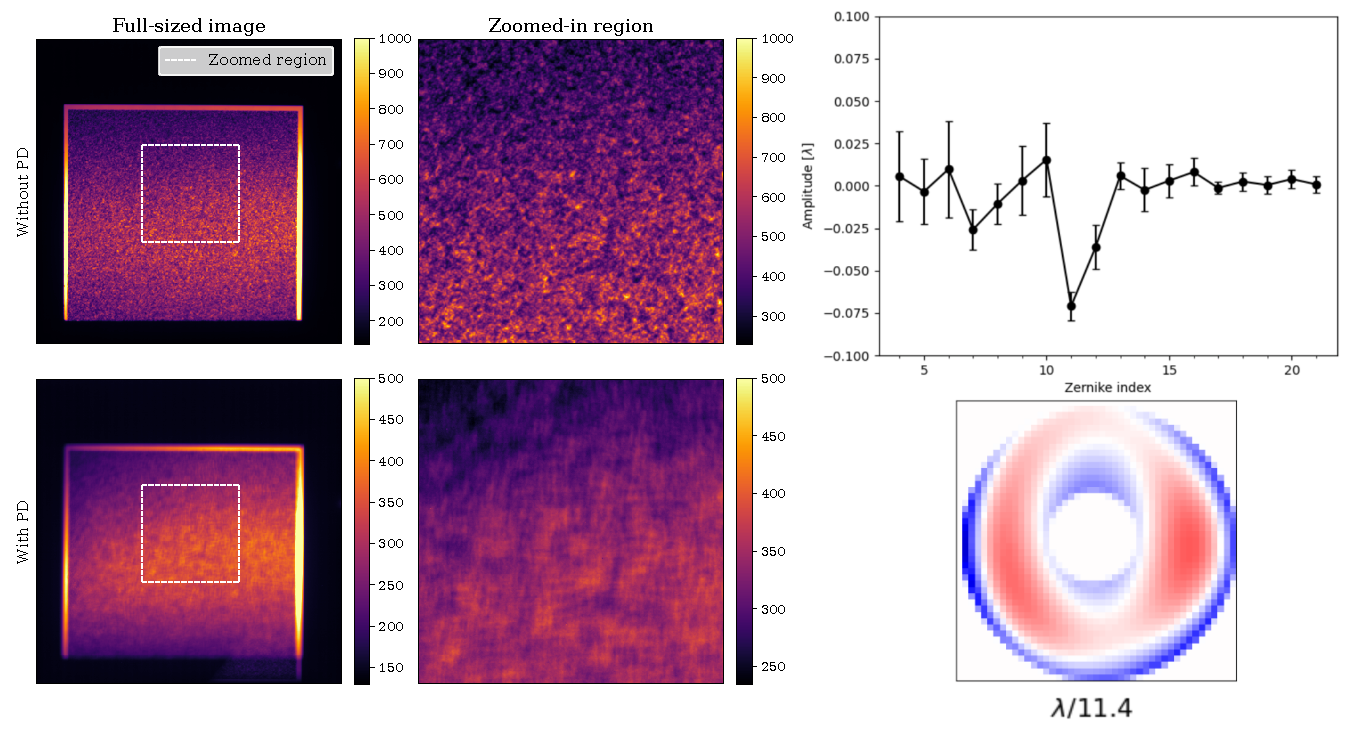
\includegraphics[width=\textwidth]{figures/TuMag/PD_e2e.pdf}
    \caption[E2E PD analysis of TuMag's optical performance.]{Random dot target measurements of the 517 nm pre-filter with the camera 1 and without the PD plate (left and central columns) taken during the Sunrise III AIV phase in Kiruna on April 2024. The right column shows the Zernike coefficients obtained from the PD analysis in the top panel and the 2D representation of the $W_{\text{rms}}$. The PD analysis has been carried out by F. J. Bailén, reproduced with permission.}
      \label{tumag : PD}
\end{figure}

Figure \ref{tumag : PD} shows the measurements and results of the PD analysis for the 517 nm pre-filter and the camera 1. The measurements were carried out during the final E2E tests performed at Kiruna on April 2024 using the random dot target (left and central columns of the figure). The measurements consist of 5 sets of focused-defocused pairs of images. The PD algorithm is run over a zoomed-in region of 600 pixels in sub-patches of 128x128 pixels. The mean Zernike coefficients are shown in the top right panel, where the error has been computed as the standard deviation between different sub-patches. A 2D representation of the $W_{\text{rms}}$ is also shown in the bottom right panel. 

The PD analysis indicates a small amplitude for most aberrations, with coefficients with a Zernike index higher than 15 approaching zero, except for the spherical aberration ($Z_{11}$ or $Z_4 ^0$) which is the dominant contribution to the $W_{\text{rms}}$. However, the results exhibit significant dispersion, as reflected by error bars that reach values up to 0.025$\lambda$ for the first coefficients. Both the defocus and astigmatism are low (Zernike indexes 4, 5 and 6, $Z _ 2 ^0$, $Z _ 2 ^{-2}$ and $Z _ 2 ^2$, respectively), agreeing with the results obtained from the MTF analysis which showed a good resolution in both vertical and horizontal directions. The overall $W_{\text{rms}}$ obtained from this analysis is $\lambda / 11.4$. It is important to note that the PD analysis shown here was carried out at the final stages of the calibration campaign, with TuMag mounted on the PFI with the light being fed to the instrument through the telescope and ISLiD system, whereas the MTF determination was conducted in the stand-alone AIV phase, without the aberrations introduced by these systems. Nevertheless, both analyses agree on a WFE better than $\lambda / 10$, indicating very high optical quality, despite the fact that the FPI of TuMag operates in a collimated configuration, which is known to degrade optical performance \citep{ghosts-etalon}.

\subsubsection{Spectral performance.}

TuMag is fed with an already spectrally-filtered light where the unwanted regions of the solar spectrum are eliminated.  Then, the instrument filters the wavelengths a second time employing a second narrow-band pre-filter that is tuned to the three selected spectral lines. Finally, the LiNbO$_3$ Fabry-Pérot etalon is in charge of selecting a very narrow band around specific wavelengths along the spectral lines. The narrow-band pre-filter and the etalon are critical to TuMag's spectroscopic performance and require careful evaluation during calibration.

The three TuMag pre-filters were custom-manufactured by Materion$^{TM}$ and have a full width at half maximum (FWHM) close to 1 nm. They are centered near the rest wavelength of the three spectral lines at normal incidence, with a peak transmission exceeding 80\% in all cases. Each pre-filter was tuned by adjusting the incidence angle to align the peak transmission wavelength with the spectral line rest wavelength. This process was performed using a coelostat at the INTA facilities, where the rest positions in volts of the spectral lines were determined. The Fe I 5250.2 \r{A} line was found at 2129 V, the Fe I 5250.6 \r{A} line at -2507 V, and the Mg I $b_2$ 5172.7 \r{A} line at -2245 V. While this tuning was successful, particularly for the iron lines, the spectral position of the pre-filters was found to be highly sensitive to illumination conditions. This sensitivity was evident from the shifts observed in the pre-filter measurements during the various stages of the assembly process. As illustrated in the left column of Fig.~\ref{fig_tumag: spectroscopic_results}, the variation in the spectral position of the pre-filters is not sufficient to cause the spectral line to be blocked by the pre-filter, but it may result in the spectral line falling on the wing of the pre-filter during observations.

\begin{table}
    \centering
   \begin{tabular}{cc}
    \hline
    \hline
    Property & Value \\
    \hline
    Reflectivity & 0.892 \\
    Thickness & 281 $\mu$m\\
    FWHM (double-pass) & 0.87 m\r{A}\\
    Tuning Constant & 3300 V/\r{A}\\
    \hline
    \hline
    \end{tabular}
    \caption{Tumag Fabry-Pérot specifications. The FWHM has been computed from the theoretical transmission profile of a collimated etalon with the reflectivity, and thickness provided in this table. See section \ref{susec_etalon_theory: collimated} for details in the analytical model of FPIs.}
    \label{table: Tumags etalon}
\end{table}

\begin{figure}
    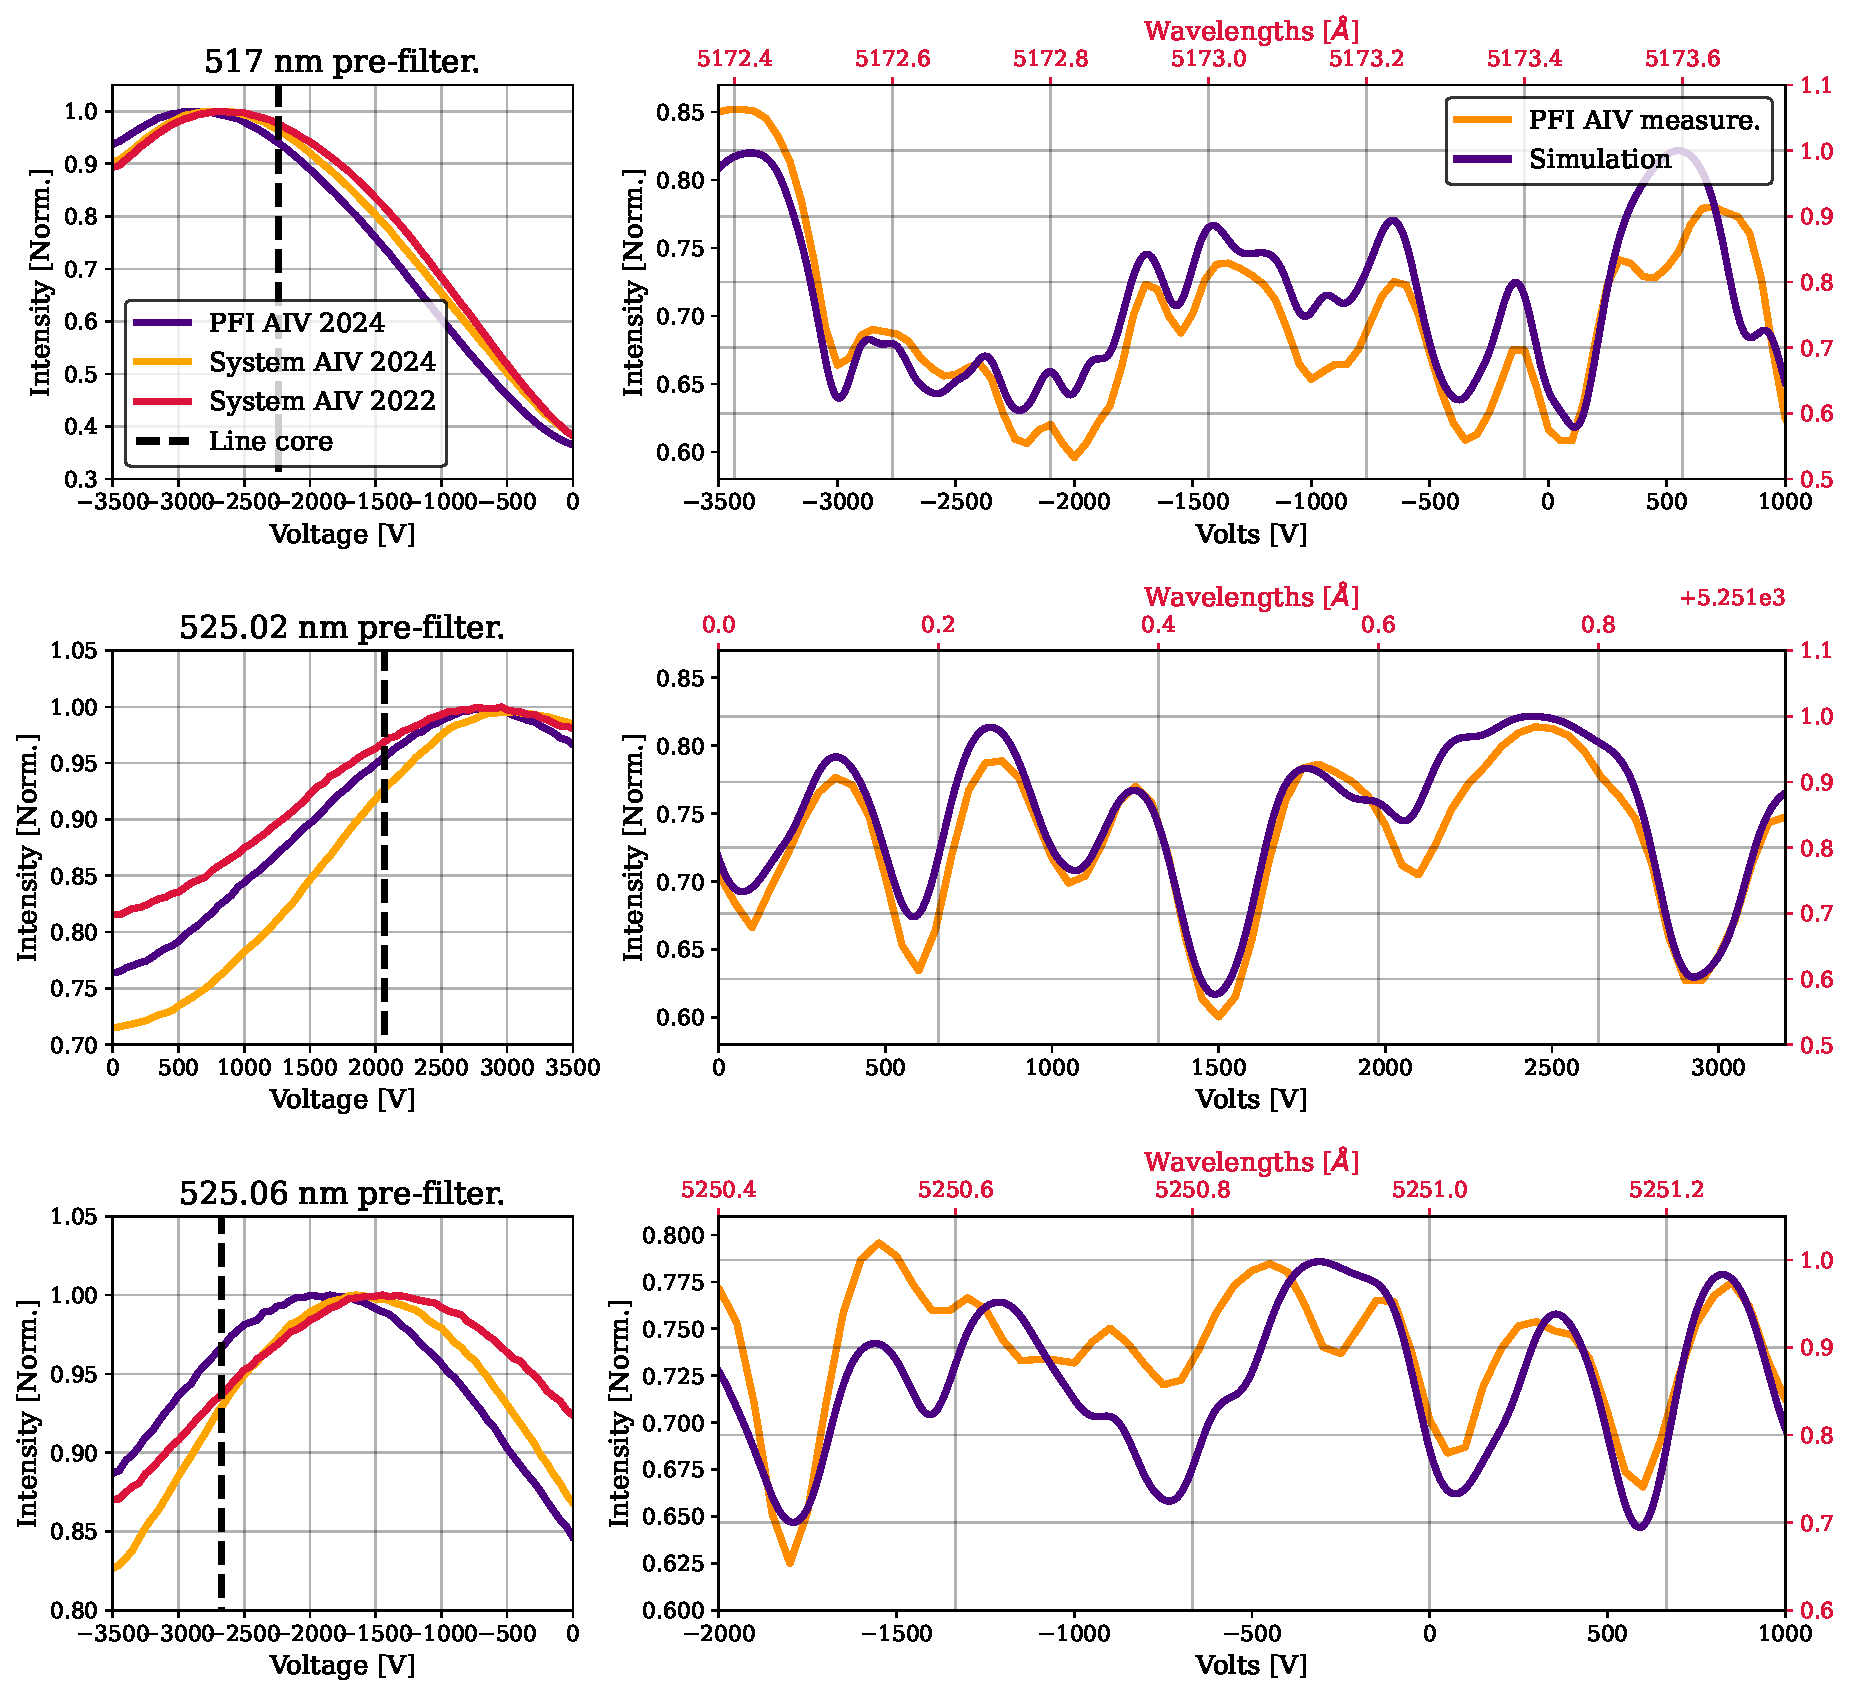
\includegraphics[width=\textwidth]{figures/TuMag/Spectroscopic_calibration.pdf}
    \caption[TuMag's spectral calibration]{
      TuMag spectroscopic calibration results. Each row shows results for the 517 nm, 525.02 nm and 525.06 nm pre-filters, from top to row. The left column shows measurements of the pre-filters carried out with a flat LED on different stages of the AIV phases. The right column shows the fit of the I$_2$ cell observation with a simulation employing an etalon with a reflectivity of 0.892 (FWHM$\sim 0.87$). Note that the absolute value of the wavelengths of the simulation (red axis) might be shifted with respect to real values due to unknown conditions of the reference.   
      \label{fig_tumag: spectroscopic_results}}
\end{figure}

TuMag etalon (see Table \ref{table: Tumags etalon}) operates in a collimated setup with a transmission profile with a FWHM of 0.87 pm (in the double-passs configuration), thus achieving a spectral resolution that exceeds the required 0.9 pm. Observations of a iodine cell illuminated with a diode were conducted to verify the transmission profile's shape and accurately assess the tuning constant. The right column of Fig.~\ref{fig_tumag: spectroscopic_results} presents, in orange, the iodine cell measurements obtained during the assembly, integration, and verification (AIV) phase of TuMag's integration into the PFI platform, which took place at the Max Planck Institute for Solar System Research (MPS) in Göttingen, Germany, in November 2023. Additionally, the dark blue line in the figure represents a simulation of the iodine spectrum observations. This simulation was generated using an analytical model of the transmission profile of collimated etalons (see section \ref{susec_etalon_theory: collimated} for a detailed overview of the model). The results confirm that the spectral resolution achieved in the iodine cell observations is consistent with the estimated 0.87 pm resolution. Furthermore, these observations enabled the calculation of the etalon's tuning constant by identifying the corresponding line cores between the simulation and observation and applying a least squares fitting to establish the relationship, which was measured in 3300 V/\r{A}.

\begin{figure}[t]
    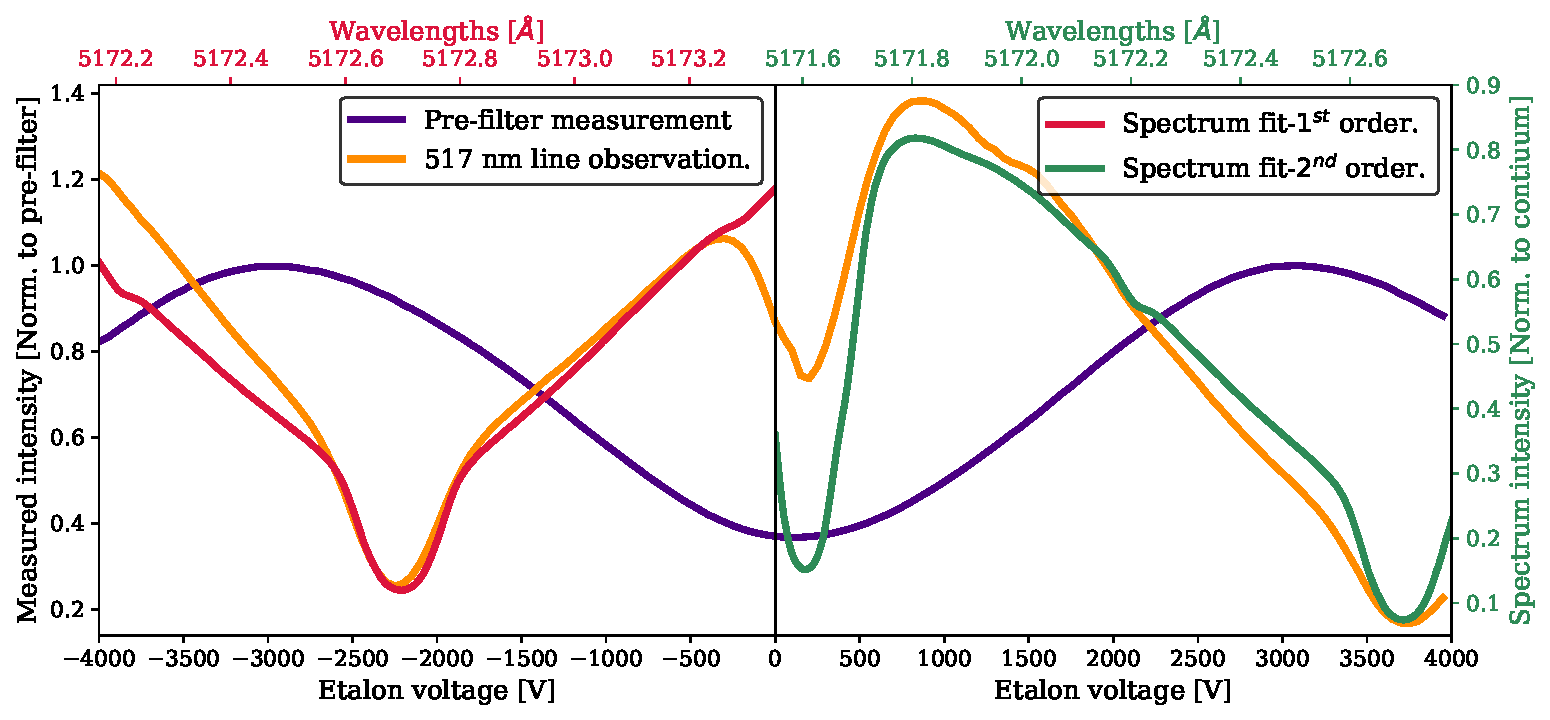
\includegraphics[width=\textwidth]{figures/TuMag/secondorder.pdf}
    \caption[Etalon's second order in magnesium measurements.]{
      Results of the spectroscopic calibration during the end-to-end calbrations of the AIV phase of 2021. The dark blue curve represents the measurement of the 517 nm pre-filter, alongside an observation of the magnesium line using the coelostat at INTA facilities, shown in orange. Two different fits of the solar spectrum are overplotted on the figure. The red line represents a fit to the primary etalon order (negative voltages), while the green line corresponds to a fit to the second etalon order (positive voltages).      
      \label{fig_tumag:second-order_cont}}
\end{figure}

An observation of the solar spectrum with the 517 nm pre-filter, conducted at INTA facilities in December 2021 during the end-to-end calibration tests, is presented in Fig.~\ref{fig_tumag:second-order_cont}, along with the corresponding pre-filter measurement. The magnesium line core is detected at approximately -2200 V using the primary order of the etalon and reappears around 3750 V with a secondary order. The solar spectrum\footnote{Taken from the Kitt Peak FTS-Spectral-Atlas \citep{fts}} is shown twice, with the magnesium core fitted to both orders. These results reveal significant contamination from the secondary order near the pre-filter's minimum transmittance. At around 0 volts, the observed spectrum (orange line) is a composite of contributions from both the primary (red line) and secondary (green line) orders, where the transmittance is diminished due to the presence of a solar line observed through the second order. The removal of this contribution is one of the steps to be performed by the data correction pipeline. This contamination is particularly relevant for data processing, as continuum measurements of the magnesium line are typically conducted at -80 V. The broader profile of the magnesium line necessitates continuum measurements farther from the line core, making it more susceptible to this contamination. In contrast, the narrower iron lines do not require such extensive offsets for continuum measurements and are thus less affected.

\subsubsection{\label{sect:tumag_cal polarimetric}Polarimetric performance.}

TuMag modulates the incoming light through a PMP composed of two LCVRs. These devices can modify the phase retardance induced to the light that goes through them by changing the alignment of their molecules when subject to a voltage. Their advantages for airborne instruments lie in their lightweight and compact design, the low voltage required for operation ([$0 - 10$]V), and their efficiency in producing either four linearly independent modulation states for full-Stokes polarimetry or only two states for measuring the longitudinal component of the magnetic field through Stokes V. This versatility is a specific advantage of LCVRs, not found in quarter-waveplate-based PMPs \citep{pmp-advantages}.

\begin{table}
    \centering
   \begin{tabular}{cc|cccc|cc}
    \hline
    \hline
     & & \multicolumn{4}{c}{Vectorial} & \multicolumn{2}{|c}{Longitudinal}  \\
     Spectral lines & Modulation & I1 & I2 & I3 & I4 & I1 & I2 \\
    \hline
    525 \& 517 nm & LCVR1 retardance  & 225$^\circ$  & 225 & 315$^\circ$ & 315$^\circ$ & 180$^\circ$  & 180$^\circ$\\
    525 \& 517 nm  & LCVR2 retardance  & 234.74$^\circ$ & 125.26$^\circ$ & 54.74$^\circ$ & 305.26$^\circ$ & 90$^\circ$ & 270$^\circ$ \\
    \hline
    525 nm & LCVR1 voltage & 2.291 & 2.533 & 1.992 & 1.947 & 2.761 & 2.761 \\
     & LCVR2 voltage & 2.375 & 3.360 & 6.433 & 2.016 & 4.723 & 2.186 \\
    \hline
    517 nm & LCVR1 voltage & 2.343 & 2.580 & 2.031 & 1.972 & 2.797 & 2.797\\
     & LCVR2 voltage & 2.371 & 3.416 & 6.548 & 2.051 & 4.77 & 2.206\\
    \hline
    \hline
    \end{tabular}
    \caption{Tumag LCVR retardances and corresponding voltages for both modulation schemes and the three pre-filters. Note that a single value is provided for both iron pre-filters.}
    \label{table: polarimetric configs}
\end{table}

TuMag's polarimetric measurement approach is divided into the two modulation schemes already mentioned: vectorial and longitudinal. In the vectorial scheme, four linearly independent modulation states are generated in rapid succession by the PMP, enabling the calculation of the full Stokes vector. Conversely, the longitudinal approach generates only two modulation states, providing information on just two components. This modulation is designed to compute Stokes V by determining the quantities $I\pm V$.

\begin{figure}[t]
    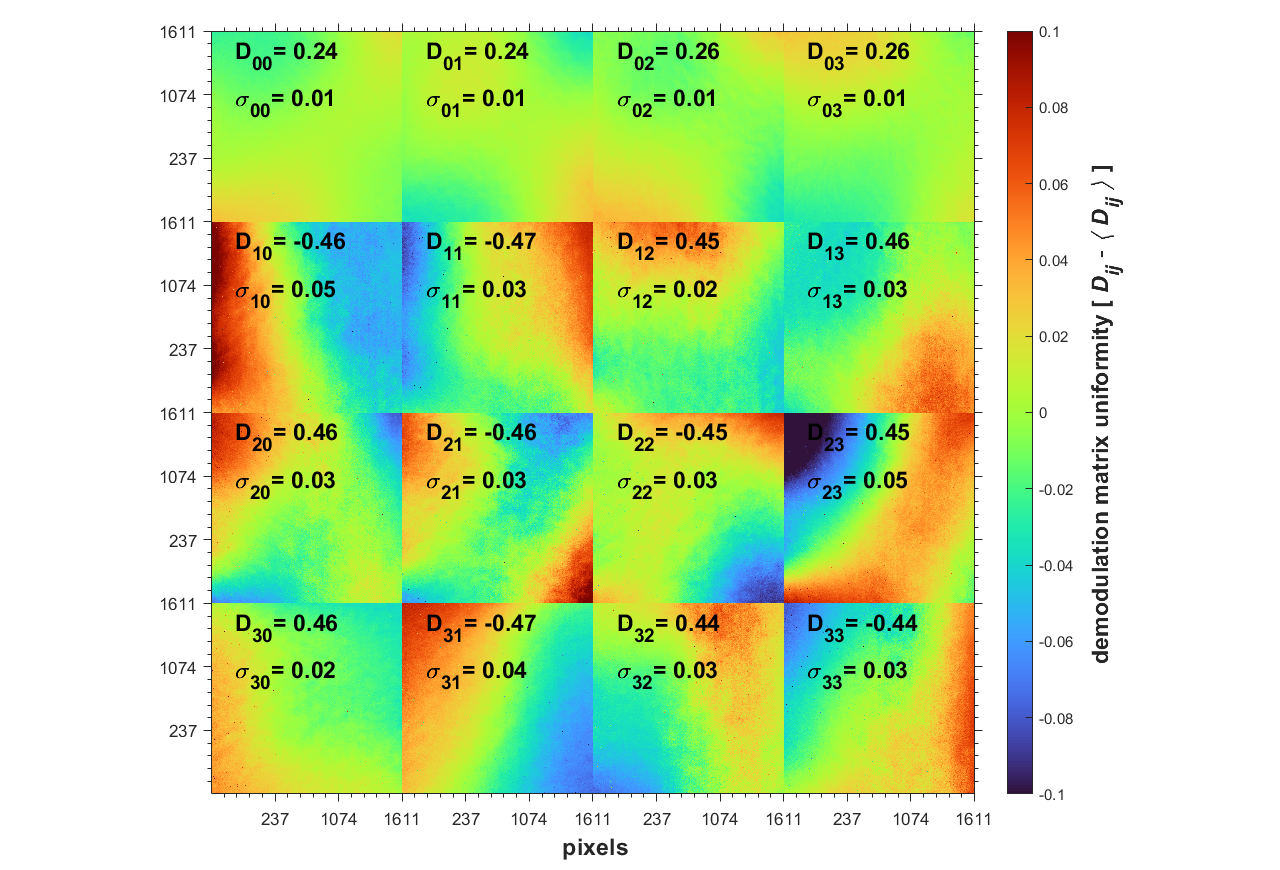
\includegraphics[width=\textwidth]{figures/TuMag/Pol_efficiencies_map.png}
    \caption[TuMag's polarimetric efficiencies.]{Polarimetric efficiencies for camera 1 and the three pre-filters (from top to bottom, the different rows show the results for 517 nm, 525.02 nm, and 525.06 nm). The different columns correspond to the efficiencies of the different Stokes components. The colormap measures the differences in efficiencies along the FoV. Results obtained during the E2E tests performed at INTA in December 2021, during the stand-alone AIV phase. Figure taken from \citep{tumag}, reproduced with permission. Analysis performed by INTA. \label{fig_tumag:pol eff maps}}
\end{figure}

Both modulation schemes are required to operate under an optimal modulation scheme. Such a scheme is defined by a modulation matrix with the following polarimetric efficiencies: $\varepsilon _{opt} \leq  [1, \frac{1}{\sqrt{3}}, \frac{1}{\sqrt{3}}, \frac{1}{\sqrt{3}}]$. The selected modulation scheme was based on the retardances outlined in Table \ref{table: polarimetric configs}. A thorough calibration of the liquid crystal variable retarders (LCVRs) was conducted to accurately determine the voltages necessary to produce the specified retardances \citep{fine-tunin}.

Considerations on the (S/N) are critical for ensuring the required polarimetric sensitivity. Achieving a S/N of $10^3$ in the Stokes measurements imposes a requirement of $S/N \approx 1300$  for each modulation measurement per camera. This calculation assumes near-optimal polarimetric performance, and takes into account the dual-beam polarimetry technique, which increases the S/N by a factor of $\sqrt{2}$ when combining data from the two cameras. A single shot of the cameras is insufficient to reach these S/N values, as the sensors do not have enough capacity in their electron wells. To address this, multiple exposures are captured and subsequently summed during each observation. This \textit{accumulation} strategy, extensively tested and employed in various polarimeters (e.g., \citealt{accs1}, \citealt{accs2}, \citealt{accs3}), has proven compatible with image reconstruction techniques \citep{accs-image1, accs-image2}. It allows for adjusting S/N levels depending on the scientific objectives of the observation, balancing between velocity and polarimetric sensitivity.

However, in order to fulfill the polarimetric sensitivity requirements, the modulation matrix of the instrument must be carefully addressed during the polarimetric calibrations. Any deviation in the computation of the modulation matrix, will introduce spurious signals in the polarization measurements, known as cross-talk. The polarimetric calibration involves a series of measurements using a light beam with a known polarization state, generated by a rotating linear polarizer and a rotating quarter-waveplate. By varying the positions of these two devices, 40 different input polarization states were produced and measured with the three pre-filters. These measurements allowed for the precise determination of the modulation matrix by solving the system of Eqs. \eqref{eq_spectro_theory: stokes_linear_comb} through a least-squares method that employs the 40 generated states. The modulation matrices for both cameras (indicated through the subindex) and all pre-filters that were determined through this process during the polarimetric E2E tests conducted at the Sunrise III AIV phase in Kiruna, Sweden, in 2022, are:
\[
\begin{matrix}
M_0 ^{517} = \begin{bmatrix}
            0.951 & -0.612 & 0.474 & 0.459 \\
            0.955 & -0.331 & -0.758 & -0.382 \\
            1.058 & 0.456 & 0.562 & -0.712 \\
            1.036 & 0.747 & -0.260 & 0.600
            \end{bmatrix}
& \quad
M_1 ^{517} = \begin{bmatrix}
            1.054 & 0.763 & -0.394 & -0.524 \\
            1.036 & 0.497 & 0.793 & 0.306 \\
            0.953 & -0.282 & -0.475 & 0.683 \\
            0.958 & -0.585 & 0.320 & -0.613
            \end{bmatrix}
\\ \\
M _ 0 ^{525.02} = \begin{bmatrix}
    0.954 & -0.694 & 0.406 & 0.414 \\
    0.969 & -0.390 & -0.803 & -0.368 \\
    1.042 & 0.418 & 0.495 & -0.705 \\
    1.035 & 0.710 & -0.266 & 0.612
    \end{bmatrix}
& \quad
M _ 1 ^{525.02} = \begin{bmatrix}
    1.059 & 0.771 & -0.449 & -0.433 \\
    1.024 & 0.449 & 0.723 & 0.335 \\
    0.965 & -0.344 & -0.543 & 0.650 \\
    0.953 & -0.606 & 0.191 & -0.641
    \end{bmatrix}
\\ \\
M _ 0 ^{525.06} = \begin{bmatrix}
    0.951 & -0.687 & 0.403 & 0.424 \\
    0.962 & -0.373 & -0.800 & -0.339 \\
    1.048 & 0.415 & 0.500 & -0.728 \\
    1.038 & 0.736 & -0.236 & 0.601
    \end{bmatrix}
& \quad
M _ 1 ^{525.06} = \begin{bmatrix}
    1.060 & 0.777 & -0.403 & -0.463 \\
    1.032 & 0.471 & 0.754 & 0.290 \\
    0.960 & -0.306 & -0.497 & 0.681 \\
    0.948 & -0.620 & 0.205 & -0.619
    \end{bmatrix}
\end{matrix}
\]

The results of the polarimetric calibration performed during the end-to-end (E2E) tests at INTA in December 2021 are presented in Figure \ref{fig_tumag:pol eff maps}. The figure shows the results for camera one; however, camera two demonstrated nearly identical efficiencies. The polarimetric efficiencies across the entire field of view (FoV) exceed the required thresholds $\varepsilon _{req} \geqslant [0.95, 0.45, 0.45, 0.45]$, and approach the optimal values. Furthermore, efficiency variations along the FoV are generally low, with standard deviations lower than 0.01. This homogeneity of the polarimetric performance should make the data reduction easier as no special treatment is required for specific regions.  